%% ID: phil_block_friction
%% TITLE: Block on a rough table
%% TYPE: question
%% QUESTIONTYPE:  numerical
%% CONCEPTS: forces, friction
%% VIDEOS: 
%% LEVEL: 3
%% TOPIC: mechanics/statics
%% ORDER: 5

\begin{problem}[Phil_block_friction]
{\question{A block is being pulled along a rough table at constant speed by a horizontal force \vari{F}. It has mass \valuedef{m}{2}{kg} and the coefficient of friction between the block and the table \valuedef{\mu}{0.5}{}. Use \valuedef{g}{9.8}{m s\sup^{-2}}. Find \vari{F}.}}
{\textit{Created for the Rutherford School Physics Project by PS.}}
{\answer{\valudef{F}{9.8}{N}}
\begin{figure}
	\centering
	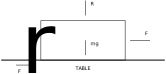
\includegraphics[width=0.4\textwidth]{Statics_block_friction}
	\caption{}
	\label{fig:Statics_block_friction}
\end{figure}
There are four forces acting on the block, as shown in Figure \ref{fig:Statics_block_friction}: the force $F$, its weight \vari{mg}, the reaction force from the table \vari{R}, and the frictional force $F\s{r}$ opposing the motion. As the block is moving at constant speed, i.e. not accelerating, we can resolve these forces. Resolving vertically on the block gives us:
\begin{equation*}	R = mg	\end{equation*}
Resolving horizontally:
\begin{equation*} F = F\s{r}	\end{equation*}
As the block is moving, we know that the friction must be at a maximum value, so $F\s{r} = F\s{r max} = \mu R$. Therefore:
\begin{equation*} F = \mu R = \mu mg	\end{equation*}
Substituting in $\mu = 0.5$, $m = 2$ and $g = 9.8$:
\begin{equation*}	F = 0.5 \times 2 \times 9.8 = 9.8\textrm{ N}	\end{equation*}
}
\end{problem}